\chapter{Collider Phenomenology}
In this chapter, we will discuss how to connect theory and experiment. We will begin by connecting scattering amplitudes and physically observed cross sections, after which we will briefly discuss detector components of the LHC, and then move on to the question of how we establish statistical significance given experimental data from detectors.

% Scattering amplitudes and cross sections
To observe physics at subatomic length scales, it is necessary to produce interactions on those scales. This requires colliding particles at speeds close to the speed of light. The energy of these collisions is so high that not only do the colliding particles scatter off of each other, but new particles can be created as well. 
The physical observable at particle colliders is a quantity known as the scattering cross section, denoted by $\sigma$. It is defined by the relation
\[R = \sigma\mathcal{L}\]
where \emph{R} is the rate of collisions per unit time, and $\mathcal{L}$ is the luminosity of the collider, that is, the number of particles passing through some cross-sectional area per unit time. The scattering cross-section $\sigma$ contains information about both the kinematics and the dynamics of the collision event, through its dependence on the scattering amplitude, $\mathcal{M}$. Thus, the typical quantities of interest are the \emph{differential} cross sections, $d\sigma/dx$, where \emph{x} represents some kinematic parameter. 
Particle colliders can broadly be classified as lepton or hadron colliders. Each one has its advantages and disadvantages. Lepton colliders have cleaner signals than hadron colliders due to the lack of large QCD backgrounds. On the other hand, hadron colliders are able to reach much larger center-of-mass energies. This is because leptons, when forced along a circular path, lose large amounts of energy via synchrotron radiation. In this work, we will focus on the phenomenology of hadron colliders, both present and future.
\section{Detector design for hadron colliders}
Particle detectors can be thought of as sophisticated videocameras with extremely high framerates. Conversely, the digital cameras that we use in our daily lives can be thought of as particle detectors, except designed for only one kind of particle, the photon. The response of a detector to an incident particle can take on a variety of forms. In a Geiger-Muller tube filled with an inert gas, an energetic particle will lead to the the brief ionization of a large fraction of the gas molecules, followed by recombination. This is manifested as an electrical pulse. The analogue of this process in a solid-state detector (such as the ones used in regular digital cameras) is the creation of a large number of electron-hole pairs in response to an energetic incident particle. The design of a particle detector will be based upon the particles it aims to detect as well as the desired precision and accuracy. Since the Large Hadron Collider is currently the epicenter of the experimental particle physics world, we will restrict our discussion to hadron colliders.
At the Large Hadron Collider at CERN, the two major experiments are ATLAS (A Toroidal LHC Apparatus) and CMS (Compact Muon Solenoid). The detectors used by these experiments differ slightly in construction, but essentially probe the same physics. The common components of these detectors are the following. 
\paragraph{Tracking chamber}
The innermost part of the detector is the tracking chamber. It consists of layers of solid-state detectors that can accurately measure the paths of charged particles that are formed in the particle collision events. The presence of a strong magnetic field bends the paths of these particles, and enables us to learn about their charge and mass.
\paragraph{Calorimeter(s)}
If a particle is energetic enough to go beyond the tracking chamber, it enters the calorimeter region. A calorimeter consists of materials dense enough to completely absorb the energy of an incident particle and stop it in its tracks. At ATLAS and CMS, the calorimeter is actually a combination of two layers that are designed to stop different particles. The electromagnetic calorimeter is designed to measure the energy of electrons and photons, while the hadronic calorimeter is designed to stop (and you might have guessed this already) hadrons. 
\paragraph{Muon Detectors} The muon, being about 200 times heavier than the electron, experiences much less energy loss through bremsstrahlung, and is able to bypass the tracking chamber and calorimeter layers. For this reason, muon detectors form the outermost layer of a particle detector.
A transverse slice of the CMS detector is shown in \autoref{fig:CMS_slice}. It shows a transverse slice of the CMS detector, with the trajectories taken by different kinds of particles.
The specific design of a detector depends upon the vision of the collaboration running it. With a finite construction and operation budget, tradeoffs must inevitably be made. Although ATLAS and CMS are both state of the art multipurpose detectors, they each have their strengths and weaknesses relative to each other based upon different sets of priorities. For this reason, we do not provide specific details about their construction, and instead point the reader to \citep{Froidevaux2006} for a detailed review.
For our purposes, the features of the collision events that we use to perform our analyses (particle momentum, missing transverse energy, etc.) can be measured with either of these detectors.
\begin{figure}[h]
  \begin{sidecaption}
    {Transverse slice of the CMS detector, showing the paths of various particles. Source: \citep{CMS_Slice}}
    \centering
    \includegraphics[trim={0 0 0 4cm},clip,width=\textwidth]{images/CMS_slice}
  \end{sidecaption}
  \label{fig:CMS_slice}
\end{figure}
\paragraph{Trigger} As mentioned in \autoref{ch:introduction}, there are hundreds of millions of collisions every second at the LHC. Recording and analyzing all of these events would be impractical, given that most of the collisions simply involve small deflections. What we are really interested in are the \emph{hard} collisions, with the final state particles having a high amount of momentum in the transverse plane. To filter out the uninteresting events, we need a \emph{trigger} - that is, a condition that an event must satisfy to be stored for further analysis. For example, in \autoref{ch:DM_100_TeV}, we choose to trigger on a \emph{hard} lepton, that is, one with a high transverse momentum.
\paragraph{Invisibles} An important point to note is that certain particles, such as neutrinos and dark matter candidates, escape the detector entirely, leaving no energy deposits. The existence of one of these `invisible' particles in a collision event can only be inferred from an observed imbalance of momenta of the final state particles in the transverse direction. Thus, for analyses involving neutrinos or dark matter, the kinematic quantity known as \emph{missing transverse energy}, denoted by $\slashed{E}_T$, is of utmost importance.

\section{Anatomy of a collider analysis}
At its heart, the goal of a collider analysis is to compare the predictions of the SM and BSM theories with actual experimental data, and estimate the level of compatibility between them. To do this well, we need precise theoretical predictions of the differential cross sections that we can expect to see at the collider. This is done with the help of Monte Carlo methods and detector simulations, as described below. 
\subsection{Parton-level event generation}
The cross section for a generic process with particles 1 and 2 colliding to produce a set of particles \emph{X} is the final state is given by the integral of the scattering amplitude for the process, $|\mathcal{M}_{12\rightarrow X}|$ over the phase space of \emph{X}\sidefootnote{Here we omit the form factors that would come into play at a hadronic collider, without affecting our narrative.}:
\[\sigma_{12\rightarrow X} = \int d\Pi_X|\mathcal{M}_{12\rightarrow X}|^2\]
In general, these integrals do not have a closed form solution, and so we must resort to numerical integration. The simplest Monte Carlo integration method involves uniformly sampling points within the limits of integration, and testing whether they lie under the `curve' specified by the integrand. The fraction of points that pass this test, multiplied by the volume of this `bounding box' specified by the integration limits, is the definite integral. This is called the \emph{acceptance-rejection} method. It is difficult to view in four dimensions, but not too hard to grasp in one or two dimensions - see \citep{Pyarelal2011} for a brief overview and implementation. However, this is not the most efficient method for performing Monte Carlo integrals - the programs MadGraph5 and MadEvent \citep{Alwall2014} do this in more sophisticated ways, iteratively determining the roughly most important regions of phase space and concentrating the sampling within those regions. These `points' are simply the particle collision events themselves, with coordinates given by the four-momenta of the final state particles. 
\subsection{Showering and hadronization}
At hadron colliders, dealing with the matrix element $\mathcal{M}$ alone will not suffice. We must also take into account nonperturbative QCD effects, such as the radiation of soft gluons, and the formation of complex hadronic final states. For example, even if an energetic quark is contained in an event generated by MadEvent, it will not be detected as an elementary particle. It will radiate gluons that themselves split to form new quarks, that subsequently form bound states. This collection of hadronic bound states is termed a jet. The momentum of the jet is collinear with the momentum of the original quark from the hard scattering process. The identity of the originating quark can be determined (with a finite efficiency) from the properties of the jet. To handle these non-perturbative effects, we interface MadEvent with the program \texttt{Pythia}\citep{Sjostrand2006} which performs the steps of parton showering and hadronization.
\subsection{Detector simulation and reconstruction}
A full collider analysis carried out by experimentalists will involve detailed simulations of the detector response, using programs such as GEANT4 \citep{Agostinelli2003}. For our purposes, however, it is enough to parameterize the detector response at a higher level - for example, specifying a fixed probability for identifying a certain particle. This is done using the Delphes 3 framework \citep{DeFavereau2014a}, which provides a way to perform a fast, modular simulation of the detector response. 
\subsection{Hypothesis testing}
After signal and background samples have been generated using Monte Carlo methods and passed through a detector simulation, they are compared to actual experimental data. Doing this enables us to do one or more of the following:
\begin{itemize}
  \item Estimate some parameter, for example the mass of a particle, or a coupling strength.
  \item Set upper limits on the rate of occurrence of a process, and translating those limits into limits on the parameter space of BSM theories.
  \item Discover a new particle
  \item Compare theoretical and experimental differential cross sections using a goodness-of-fit test.
\end{itemize}
As it turns out, all of these can be subsumed into the larger framework of \emph{hypothesis testing} \citep{Heinrich}.

\section{Future circular colliders}

\begin{figure}[h]
  \begin{sidecaption}
    {Schematic diagram of the FCC ring.}
    \centering
  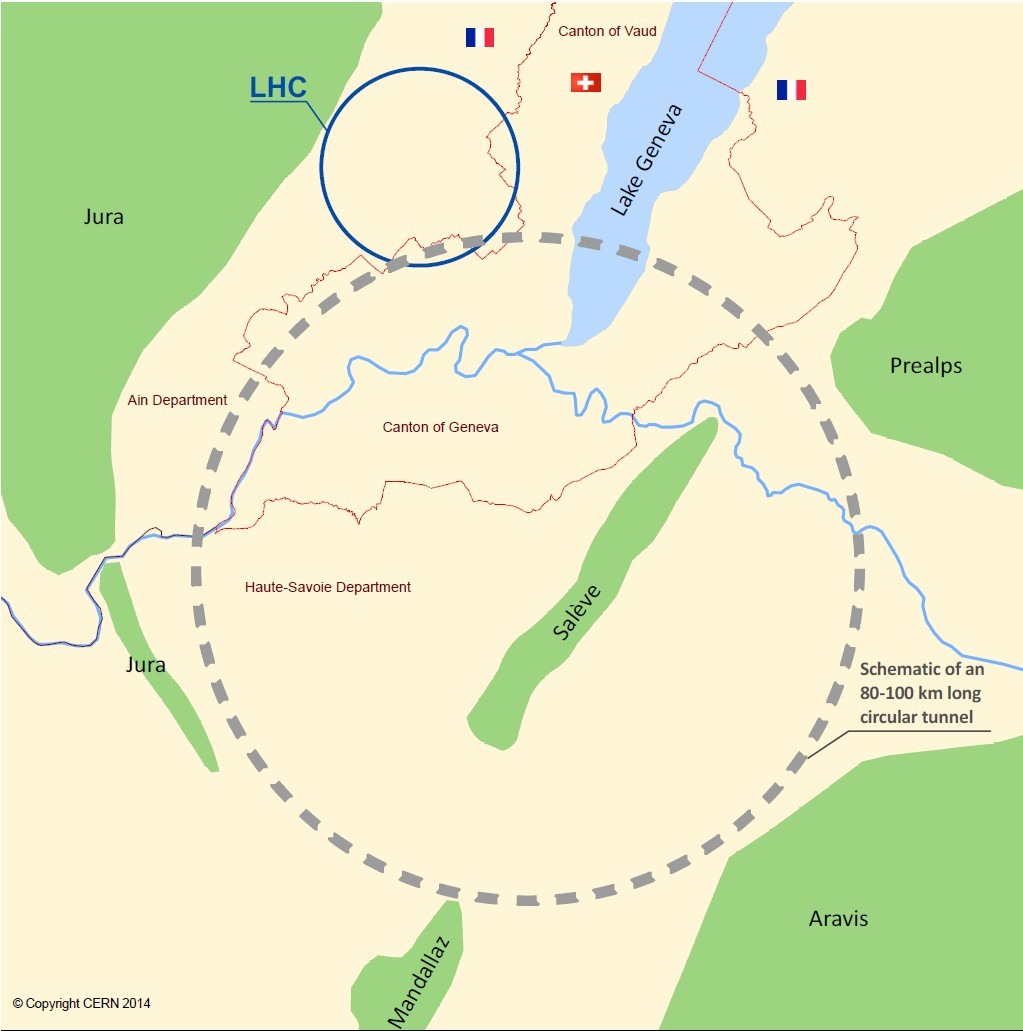
\includegraphics[width=0.9\textwidth]{images/FCC_ring_schematic}
  \end{sidecaption}
\end{figure}
\section{Statistical significance in particle physics}
